% THIS IS SIGPROC-SP.TEX - VERSION 3.1
% WORKS WITH V3.2SP OF ACM_PROC_ARTICLE-SP.CLS
% APRIL 2009
%
% It is an example file showing how to use the 'acm_proc_article-sp.cls' V3.2SP
% LaTeX2e document class file for Conference Proceedings submissions.
% ----------------------------------------------------------------------------------------------------------------
% This .tex file (and associated .cls V3.2SP) *DOES NOT* produce:
%       1) The Permission Statement
%       2) The Conference (location) Info information
%       3) The Copyright Line with ACM data
%       4) Page numbering
% ---------------------------------------------------------------------------------------------------------------
% It is an example which *does* use the .bib file (from which the .bbl file
% is produced).
% REMEMBER HOWEVER: After having produced the .bbl file,
% and prior to final submission,
% you need to 'insert'  your .bbl file into your source .tex file so as to provide
% ONE 'self-contained' source file.
%
% Questions regarding SIGS should be sent to
% Adrienne Griscti ---> griscti@acm.org
%
% Questions/suggestions regarding the guidelines, .tex and .cls files, etc. to
% Gerald Murray ---> murray@hq.acm.org
%
% For tracking purposes - this is V3.1SP - APRIL 2009

\documentclass{acm_proc_article-sp}
\usepackage{algorithm} %format of the algorithm
\usepackage{algorithmic} %format of the algorithm
\usepackage{graphics}
%%%%%%%%%%%%%%%%%%%%%%%%%%%%

\begin{document}

\title{Discussion about the Steepest Descent Method}


\numberofauthors{2}

\author{
% 1st. author
\alignauthor
Tianxing He\\
       \affaddr{SJTU ACM10}\\
       \email{cloudygooseg@gmail.com}
% 2nd. author
\alignauthor
Yuchen Fan\\
       \affaddr{SJTU ACM10}\\
       \email{fyc0624@gmail.com}
}
\date{21 December 2012}

\maketitle
\begin{abstract}
In our work, we explore the Steepest Descent method, which could be seen as an variation of the well-studied Gradient Descent method. First, we will give the exact definition of the Steepest Descent method, then we will give convergence analysis for both these two methods, which are very similar. \\
Then, through our experiment, we showed the drastic impact on the performance of the Steepest Descent method by the choice norm we use. Finally, we try to use the Hessian to automatically construct the norm, which we put the G-S descent, but sadly failed.
\end{abstract}

\keywords{Convex optimization, Steepest descent}

\section{INTRODUCTION}
In the field of solving unconstrained optimization problem, one most well-known and well-studied method, is the Gradient Descent method, we first briefly introduce the Gradient Descent, which is shown in Algorithm \ref{alg:A}.\\
In the step 2 of the Gradient Descent method, we must choose exact line search or backtracking line search, while exact line search is preferred, in our experiments we will use the backtracking line search, which is more easy to implement. The backtracking line search is shown in Algorithm \ref{alg:B}. Figure \ref{fig:back} should help to understand what it's doing, the backtracking is to prevent the step from 'going too far'.
\begin{algorithm}\caption{\label{alg:A}Gradient descent method.}
\begin{algorithmic}
\STATE \textbf{Given} a starting point $x \in \textbf{dom} f$
\REPEAT
\STATE 1. $\Delta x:=-\nabla f\left( x\right) $.
\STATE 2. \textit{Line search.} Choose step size t via exact or backtracking line search.
\STATE 3. \textit{Update.} $x:=x+t\Delta x$
\UNTIL{stopping criterion is satisfied.}
\end{algorithmic}
\end{algorithm}

\begin{figure}
        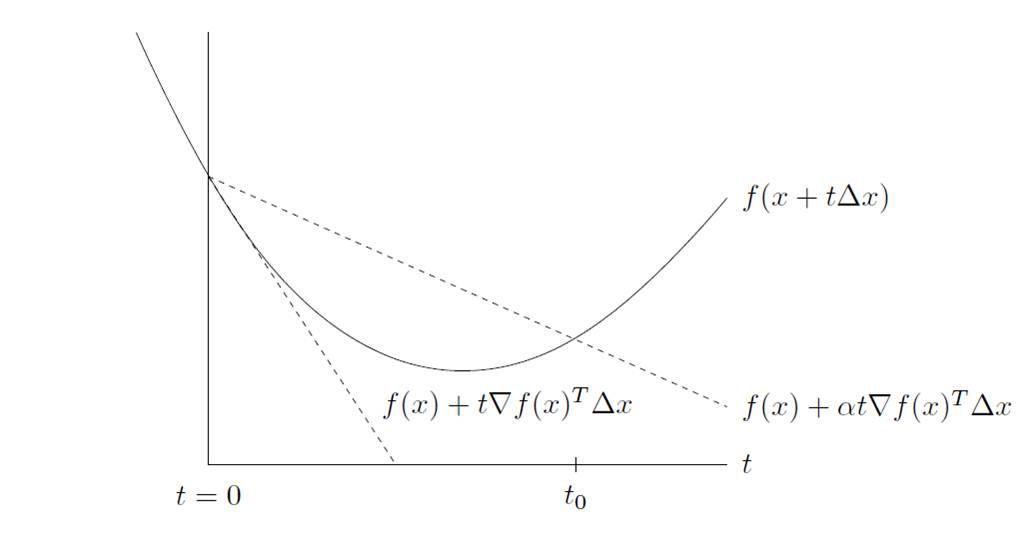
\includegraphics[width=80mm]{backtracking.jpg}
    \caption{\label{fig:back}The backtracking line search.}
\end{figure}

\begin{algorithm}\caption{\label{alg:B}Backtracking line search.}
\begin{algorithmic}
\STATE \textbf{Given} a starting point $\bigtriangleup x$ for f at $x \in \textbf{dom} f, \alpha \in (0,0.5), \beta \in (0,1)$
\STATE \textbf{While} $f(x + t\bigtriangleup x) > f(x) + \alpha t \nabla f(x)^T \bigtriangleup x$ \\
{$t = \beta t$}
\end{algorithmic}
\end{algorithm}
We have to mention due to some historical reasons the Gradient Descent is also called the Steepest Descent method\cite{avriel2003nonlinear}(Well, its direction is truly locally 'steepest'). However, the Steepest Descent method is another story.\\
In the next section, we will give convergence analysis of the Gradient Descent method, after which it should be clear that the convergence rate is highly related to the 'condition number' of the sublevel set. The Steepest Descent method proposes a way to change the condition number by introducing norms to the Gradient Descent method.\\

\section{Convergence analysis\cite{boyd2004convex}}
In this section we present a simple convergence analysis for the gradient method,
using the lighter notation $x^{+}=x+t\Delta x$for$x^{(k+1)}=x^{(k)}+t^{(k)}\Delta x^{(k)}$, where$\Delta x=-\nabla f(x)$.
We assume $f$ is strongly convex on $S$, 
so there are positive constants $m$ and $M$ such that $mI\preceq \Delta^{2}f(x)\preceq MI$ for all $x\in S$.
Define the function $\widetilde{f}:R\rightarrow R$ by $\widetilde{f}(t)=f(x-t\Delta f(x))$, \textit{i.e.},
$f$ as a function of the step length $t$ in the negative gradient direction. 
In the following discussion we will only consider $t$ for which $x-t\Delta f(x)\in S$. 
Assume the object function is strongly convex, we obtain a quadratic upper bound on $\widetilde{f}$:

\begin{eqnarray}
\widetilde{f}(t)\leq f(x)-t\left\| \nabla f\left( x\right) \right\| _{2}^{2} + \dfrac {Mt^{2}} {2}\left\| \nabla f\left( x\right) \right\| _{2}^{2}
\label{eq:9.17}
\end{eqnarray}

\subsection{Analysis for exact line search}
We now assume that an exact line search is used, and minimize over t both sides of the inequality (\ref{eq:9.18})
On the lefthand side we get $\widetilde{f}(t_{exact})$, 
where $t_{exact}$is the step length that minimizes $\widetilde{f}$. 
The righthand side is a simple quadratic, which is minimized by $t = \dfrac{1}{M},$ 
and has minimum value $f(x)−\dfrac{1}{2M}\left\| \nabla f\left( x\right) \right\| _{2}^{2}.$
Therefore we have
$$f(x^{+})=\widetilde{f}(t_{texact})\leq f(x)− \dfrac{1}{2M}\left\| \nabla f\left( x\right) \right\| _{2}^{2}.$$
Subtracting $p^{*}$from both sides, we get
$$f(x^{+})−p^{*}\leq f(x)−p^{*}−\dfrac{1}{2M}\left\| \nabla f\left( x\right) \right\| _{2}^{2}.$$
We combine this with $\left\| \nabla f\left( x\right) \right\| _{2}^{2} \geq 2m(f(x)-p^{*})$(because the object function is strongly convex) to conclude
$$f(x^{+})−p^{⋆}\leq (1-m/M)(f(x)−p^{⋆})$$. 
Applying this inequality recursively, we find that

\begin{eqnarray}
f(x^{(k)})−p^{⋆}\leq c^{k}(f(x^{(0)})−p^{⋆})
\label{eq:9.18}
\end{eqnarray}

where $c = 1 − m/M < 1$, which shows that $f(x^{(k)})$ converges to $p^{⋆}$ as $k\rightarrow \infty$. 
In particular, we must have $f(x^{(k)})−p^{⋆}\leq \varepsilon$ after at most

\begin{eqnarray}
\dfrac{log((f(x^{(0)})−p^{⋆})/\varepsilon)}{log(1/c)}
\label{eq:9.19}
\end{eqnarray}

iterations of the gradient method with exact line search. 

This bound on the number of iterations required, even though crude, 
can give some insight into the gradient method. 
The numerator,
$$log((f(x^{(0)})−p^{⋆})/\varepsilon)$$
can be interpreted as the log of the ratio of the initial suboptimality (\textit{i.e.}, gap between $f(x^{(0)})$ and $p^{⋆}$), 
to the final suboptimality (\textit{i.e.}, less than $\varepsilon$). 
This term suggests that the number of iterations depends on how good the initial point is,
and what the final required accuracy is.

The denominator appearing in the bound (\ref{eq:9.19}), $log(1/c)$, is a function of $M/m$,
which we have seen is a bound on the condition number of $\Delta ^{2}f(x)$ over $S$, 
or the condition number of the sublevel sets $\{z \| f(z)\leq \alpha\}$. 
For large condition number bound $M/m$, we have
$$log(1/c)=−log(1 − m/M)\thickapprox m/M$$,
so our bound on the number of iterations required increases approximately linearly with increasing $M/m$. 

We will see that the gradient method does in fact require a large number of iterations when the Hessian of $f$, 
near $x^{⋆}$, has a large condition number. 
Conversely, when the sublevel sets of $f$ are relatively isotropic, 
so that the condition number bound $M/m$ can be chosen to be relatively small, 
the bound (\ref{eq:9.18}) shows that convergence is rapid, 
since $c$ is small, or at least not too close to one.

The bound (\ref{eq:9.18}) shows that the error $f(x^{(k)})−p^{⋆}$ converges to zero at least as fast as a geometric series. 
In the context of iterative numerical methods, this is called linear convergence, 
since the error lies below a line on a log-linear plot of error versus iteration number.

\subsection{Analysis for backtracking line search}
Now we consider the case where a backtracking line search is used in the gradient descent method. 
We will show that the backtracking exit condition,
$$\widetilde{f}(t)\leq f(x)−\alpha t\left\| \nabla f\left( x\right) \right\| _{2}^{2}$$, 
is satisfied whenever $0 \leq t \leq 1/M$. 
First note that
$$0 \leq t \leq 1/M \Rightarrow −t+\dfrac{Mt^{2}}{2} \leq −t/2$$
(which follows from convexity of $−t+Mt^{2}/2$). Using this result and the bound (\ref{eq:9.17}),
we have, for $0 \leq t \leq 1/M$,

\begin{equation}
    \begin{array}{rcl}
        \widetilde{f}(t) & \leq & f(x)− t\left\| \nabla f\left( x\right) \right\| _{2}^{2} + \dfrac{Mt^{2}}{2}\left\| \nabla f\left( x\right) \right\| _{2}^{2} \\
        & \leq & f(x) - (t/2)\left\| \nabla f\left( x\right) \right\| _{2}^{2}\\
        & \leq & f(x) - \alpha t\left\| \nabla f\left( x\right) \right\| _{2}^{2}\\
    \end{array}
\end{equation},
since $\alpha < 1/2$. Therefore the backtracking line search terminates either with $t = 1$ or with a value $t \geq \beta/M$.
This provides a lower bound on the decrease in the objective function. 
In the first case we have
$$f(x^{+}) \leq f(x) − \alpha \left\| \nabla f\left( x\right) \right\| _{2}^{2}$$, 
and in the second case we have
$$f(x^{+}) \leq f(x) − (\beta\alpha /M) \left\| \nabla f\left( x\right) \right\| _{2}^{2}$$. 
Putting these together, we always have
$$f(x^{+}) \leq f(x) − \min\{\alpha, \beta\alpha /M\} \left\| \nabla f\left( x\right) \right\| _{2}^{2}$$, 
Now we can proceed exactly as in the case of exact line search. We subtract $p^{⋆}$ from both sides to get
$$f(x^{+})-p^{*} \leq f(x)-p^{*} − \min\{\alpha, \beta\alpha /M\} \left\| \nabla f\left( x\right) \right\| _{2}^{2}$$, 
and combine this with $\left\| \nabla f\left( x\right) \right\| _{2}^{2} \geq 2m(f(x)-p^{*})$ to obtain
$$f(x^{+})-p^{*} \leq (1 − \min\{\alpha, \beta\alpha /M\})(f(x)-p^{*})$$. 
From this we conclude
$$f(x^{(k)}) − p^{⋆} \leq c^{k}(f(x^{(0)}) − p^{⋆})$$
where
$$c = 1 - \min\{2m\alpha , 2\beta \alpha m/M\} < 1$$.
In particular, $f (x^{(k)})$ converges to $p^{⋆}$ at least as fast as a geometric series with an
exponent that depends (at least in part) on the condition number bound $M/m$. In
the terminology of iterative methods, the convergence is at least linear.

Let $||\cdot||$ be any norm on $R^n$. We define a normalized steepest descent direction(with respect to the norm $||\cdot||$) as
\begin{displaymath}
\Delta x _{nsd} = argmin\{ \nabla f(x)^Tv| ||v|| = 1\}
\end{displaymath}
Now we can give the Steepest descent method in Algorithm \ref{alg:C}.
\begin{algorithm}\caption{\label{alg:C}Steepest descent method}
\begin{algorithmic}
\STATE \textbf{Given} a starting point $x \in \textbf{dom} f$
\REPEAT
\STATE 1. Compute steepest descent direction $\Delta x _{nsd}$.
\STATE 2. \textit{Line search.} Choose step size t via exact or backtracking line search.
\STATE 3. \textit{Update.} $x:=x+t\Delta x$
\UNTIL{stopping criterion is satisfied.}
\end{algorithmic}
\end{algorithm}
To get a better understanding of the Steepest Descent Method, let's look at some examples.
\subsection{Steepest Descent for Euclidean and quadratic norms}
If  we take the norm $||\cdot||$ to be the Euclidean norm, then the steepest descent direction is simply the negative gradient.\\
Given a $P \in S^n_{++}$, now we consider the quadratic norm
\begin{displaymath}
||z||_P = (z^TPz)^{1/2} = ||P^{1/2}||_2
\end{displaymath}
The normalized steepest descent direction is given by
\begin{displaymath}
\Delta x_{nsd} = -(\nabla f(x) ^ T P ^{-1} \nabla f(x))^{-1/2} P ^{-1} \nabla f(x)
\end{displaymath}
Now we show how this direction is obtained by an interpretation via change of coordinates. Define $\overline{u} = p^{1/2} u$, so we have $||u||_P = ||\overline{u}||_2$. Using this change of coordinates, we can solve the original problem of minimizing f by solving the equivalent problem of minimizing the function $\overline{f}$, given by
\begin{displaymath}
\overline{f}(\overline{u})=f(P^{-1/2}\overline{u})=f(u)
\end{displaymath}
If we apply the gradient method to $\overline{f}$, the search direction at a point $\overline{x}$ is
\begin{displaymath}
\Delta\overline{x} = - \nabla \overline{f}(\overline{x}) = -P^{-1/2} \nabla f(P^{-1/2}\overline{x}) = -P^{-1/2} \nabla f(x)
\end{displaymath}
This gradient search direction corresponds to the direction
\begin{displaymath}
\Delta x = P^{-1/2}(-P^{-1/2}\nabla f(x)) = - P^{-1} \nabla f(x)
\end{displaymath}
for the original variable x. In other words, the steepest descent method in the quadratic norm $||\cdot||_P$ can be thought of as the gradient method applied to the problem after the change of coordinates $\overline{x} = P^{1/2} x$.
\section{Discussion and examples}
\subsection{choice of norm for steepest descent}
One important thing for the steepest descent method is to choose a good norm. In our convergence analysis, we know that the gradient method works well when the condition number of the sublevel sets are moderate, and poorly otherwise. Let's begin with the quadratic $P$-norm, we know that using the quadratic $P$-norm means that we change coordinates by $\overline{x} = P^{1/2}x$. So, a good idea would be to make the ellipsoid
\begin{displaymath}
\varepsilon = \{ x | x^TPx \leq 1\}
\end{displaymath}
be a good approximation of the shape of the sublevel set.(In other words, it gives a good approximation after appropriate scaling and translation.) \\
Let's consider the following function :
\begin{displaymath}
g_1(x_1, x_2) = e ^ {x_1 + 3x_2 -0.1} + e ^ {x_1-3x_2-0.1} + e^{-x_1-0.1}
\end{displaymath}
For all three tries, we start at point$(-0.4,1)$, and use the backtracking line search with $\alpha=0.2$, $\beta=0.8$, and let the initial step be 1, the tolerance is 0.01. For the two steepest descent tries, we choose $P_1 = \begin{array}{cc} 1/2 & 0 \\ 0 & 1/4\end{array}$ and
$P_2 = \begin{array}{cc} 1/4 & 0 \\ 0 & 1/2\end{array}$, the results are shown in Figure \ref{fig:htx1}.\\
We also add the shape of the norms on the graphs. From the results, we can clearly see that the norm $P_1$, which is a better
approximate of the sublevel set, give the best result. And we we use $P_2$, it becomes worse than the original gradient descent. \\
\begin{figure*}[hp]
        \begin{tabular}{ccc}
            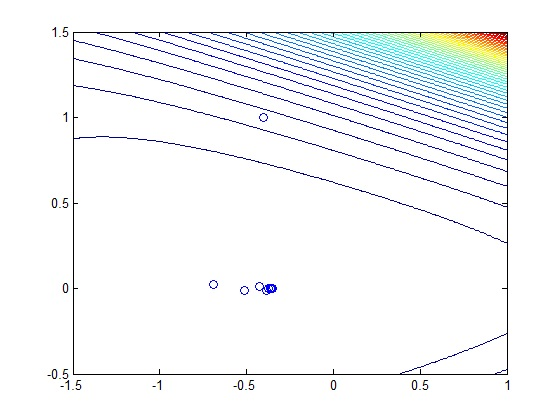
\includegraphics[width=55mm]{htx1-1.jpg} &
            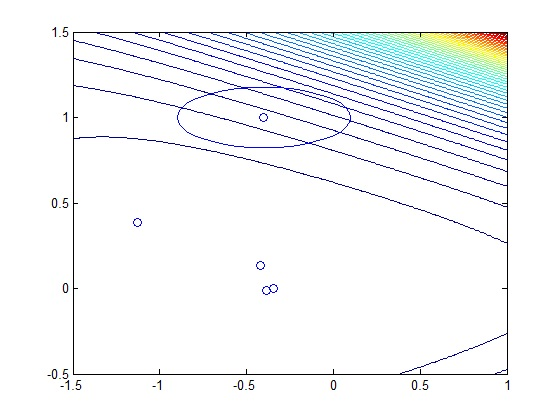
\includegraphics[width=55mm]{htx1-2.jpg} &
            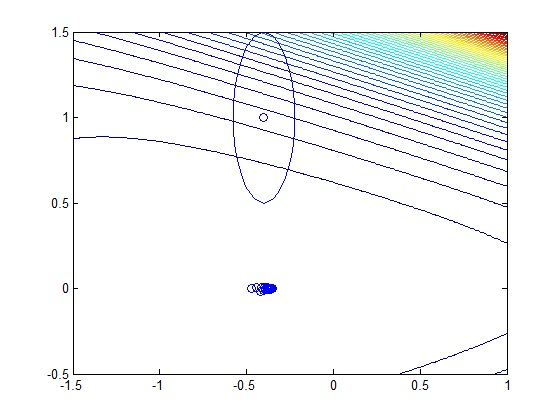
\includegraphics[width=55mm]{htx1-3.jpg} \\
            G-descent : 11 iterations &
            S-descent with $P_1$ : 6 iterations &
            S-descent with $P_2$ : 29 iterations
        \end{tabular}
    \caption{\label{fig:htx1}Three methods for $g_1$.}
\end{figure*}
To further illustrate the power of the steepest descent method, we choose a function which is exactly a ellipse:
\begin{displaymath}
g_2(x_1, x_2) = x_1 ^ 2 + 8 * x_2 ^ 2
\end{displaymath}
The result are shown in Figure \ref{fig:htx2}, from which we can see the drastic effect imposed by the choice of the norm, we omit the parameters here.
\begin{figure*}[hp]
        \begin{tabular}{ccc}
            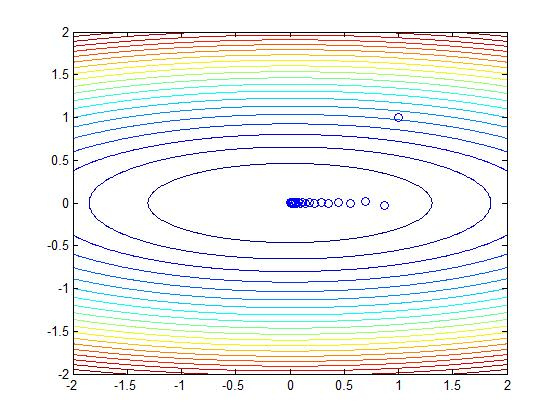
\includegraphics[width=55mm]{htx2-1.jpg} &
            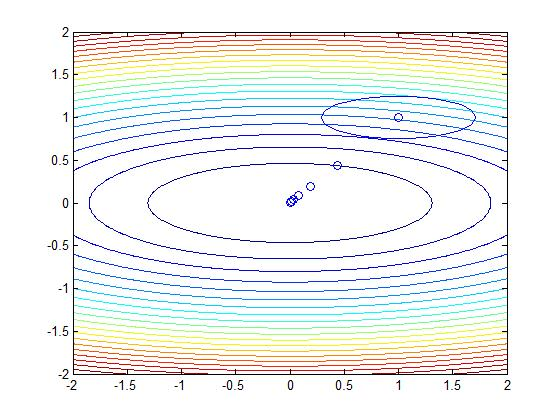
\includegraphics[width=55mm]{htx2-2.jpg} &
            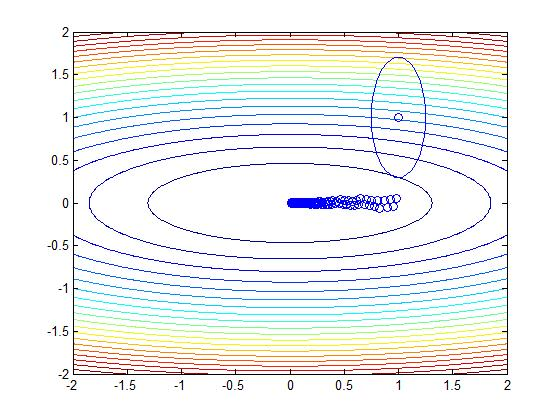
\includegraphics[width=55mm]{htx2-3.jpg} \\
            G-descent : 23 iterations &
            S-descent with $P_1$ : 10 iterations &
            S-descent with $P_2$ : 134 iterations
        \end{tabular}
    \caption{\label{fig:htx2}Three methods for $g_2$.}
\end{figure*}
\subsection{attempts to construct the norm using Hessian}
Now we know how could we use norm to aid the gradient descent method. One important issue still remains: how could we find the best norm? From the Taylor series, we know that around the local optima $x^{\star}$,
\begin{displaymath}
f(y) \approx p^{\star} + \frac{1}{2} (y - x^\star)^T\nabla^2f(x^\star)(y-x^\star)
\end{displaymath}
So we know the sublevel set near the local optima is well approximated by an elliposid. Now we try to use the Hessian as the $P$, which means, let
\begin{displaymath}
P = \nabla^2f(x)
\end{displaymath}
However, this is sometimes invalid: we need the $P$ to be semi-definite.\\
Given this insight, let's consider the simplified $g_1$
\begin{displaymath}
g_3(x_1, x_2) = e ^ {x_1 + 3x_2} + e ^ {x_1-3x_2} + e^{-x_1}
\end{displaymath}
First we want to let the $P = \nabla^2f(x)$ every step, but we failed, when we peek at the results, we found that the $P$s are really ill-presented, we concluded that the reason is that we are not near the optima.\\
To get the hessian be a good approximation, a second thought is that we can exploit the long-tail property of the descent methods, that is: The start point is (0.9,0.9), At first we set the $P$ to be the identity matrix, i.e, exactly do the gradient descent, however, when $\nabla f(x) < tolerance * 10$, we switch the $P$ to be the local Hessian, let's call this the G-S descent.
\begin{figure*}[hp]
        \begin{tabular}{cc}
            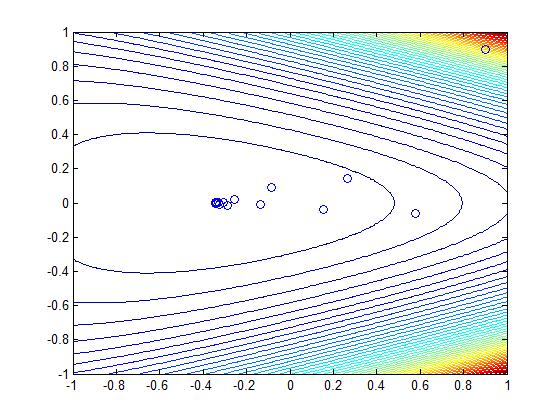
\includegraphics[width=55mm]{htx3-1.jpg} &
            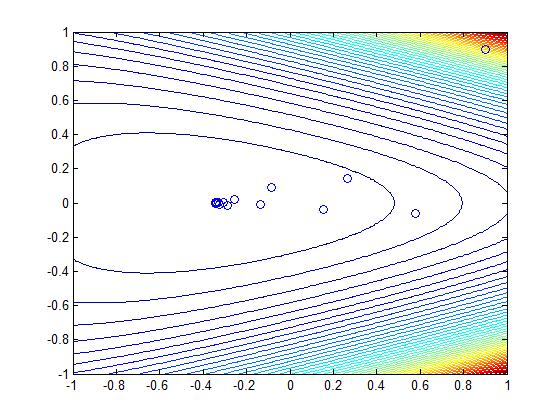
\includegraphics[width=55mm]{htx3-2.jpg} \\
            G-descent : 15 iterations&
            G-S-descent with Hessian : 19 iterations \\
        \end{tabular}
    \caption{\label{fig:htx3}Two methods for $g_3$.}
\end{figure*}
Sadly, the G-S only slow downs the process, which is not hard to understand, when the x converges to the optima, the direction of the gradient becomes stable, so the norm won't do any good. So, if we choose to use the Steepest Descent, we should use the norm we choose from the beginning.

\section{CONCLUSIONS}
In our report, we discussed the Steepest Descent method, which is an variation of the Gradient Descent method. In our convergence analysis of the Gradient Descent method, we saw that the condition number is highly related to the performance, so comes the idea of using norms. In our experiments, we illustrates that the choice of norms has a drastic impact on the performance of the Steepest Descent method, we also attempt to use the Hessian near the optima as the norm.

\bibliographystyle{unsrt}
\bibliography{htx} 

%\section{REFERENCES}
%Nonlinear Programming: Analysis and Methods Dover Publishing\\
%Convex Optimization Stephen Boyd and Lieven Vandenberghe\\
\balancecolumns
% That's all folks!
\end{document}

